% ==============================================================================================
\chapter{Dynamic strip load elastic halfspace} \label{ch:strip_load_2D}
% ==============================================================================================

% ----------------------------------------------------------------------------------------------
\section{Introduction}
% ----------------------------------------------------------------------------------------------
This benchmark compares the STEM numerical solution against the analytical solution,
where a dynamic line load is applied along the surface of an elastic half-space discretised in a plane-strain setting.

The analytical solution is presented in~\cite{Verruijt_Brinkgreve_Li_2008}.
The analytical solution provides closed-form expressions for the vertical stress along the surface of the
half-space, enabling a direct time-history comparison against the numerical model.

% ----------------------------------------------------------------------------------------------
\section{Model Description}
% ----------------------------------------------------------------------------------------------

% ..............................................................................................
\subsection{Geometry, mesh and loading}
% ..............................................................................................
The analytical solution is formulated in plane-strain conditions. To mimic this, two analyses are performed:
a two-dimensional analysis representing a strip load in plane-strain conditions, and a three-dimensional
analysis representing a strip load in a full 3D setting, where the thickness in the out-of-plane direction is set to
\qty{1}{\meter} and the displacements are fixed in the out-of-plane direction. This allows to verify that the
three-dimensional solution converges to the analytical solution.

In the two-dimensional analysis, the soil domain is modelled as a
\qty{20}{\meter} (x-direction) by \qty{10}{\meter} (y-direction) soil layer,
modelled with second-order triangular elements.

In the three-dimensional analysis, the soil domain is modelled as  a \qty{20}{\meter} (x-direction) by \qty{10}{\meter}
(y-direction) soil layer, extruded to \qty{1}{\meter} thickness in the z-direction, and modelled with second-order
 tetrahedral elements.

Both analyses use a mesh with an average element size of \qty{0.15}{\meter}.

Figure~\ref{fig:strip_mesh} illustrates the geometry and mesh adopted for the analyses.

The strip load is applied at the surface with a width of \qty{1}{\meter}.
A downward line load with magnitude \qty{1e6}{\newton\per\meter} is applied instantaneously and kept
constant during the analysed time window:

\begin{equation}
    q(t) =
    \begin{cases}
        0, & t < 0, \\
        \qty{-1000}{\kilo\newton\per\meter}, & t \geq 0.
    \end{cases}
\end{equation}

The nodes at the bottom are fully fixed, while the two vertical sides are restrained only in the normal direction
(roller boundaries) to allow vertical and tangential movement.
In the three-dimensional case, the front and back surface are prevented from moving in the
out-of-plane direction, to simulate plane-strain conditions along the extrusion axis.

\begin{figure}
    \centering
    \begin{subfigure}[t]{0.49\textwidth}
        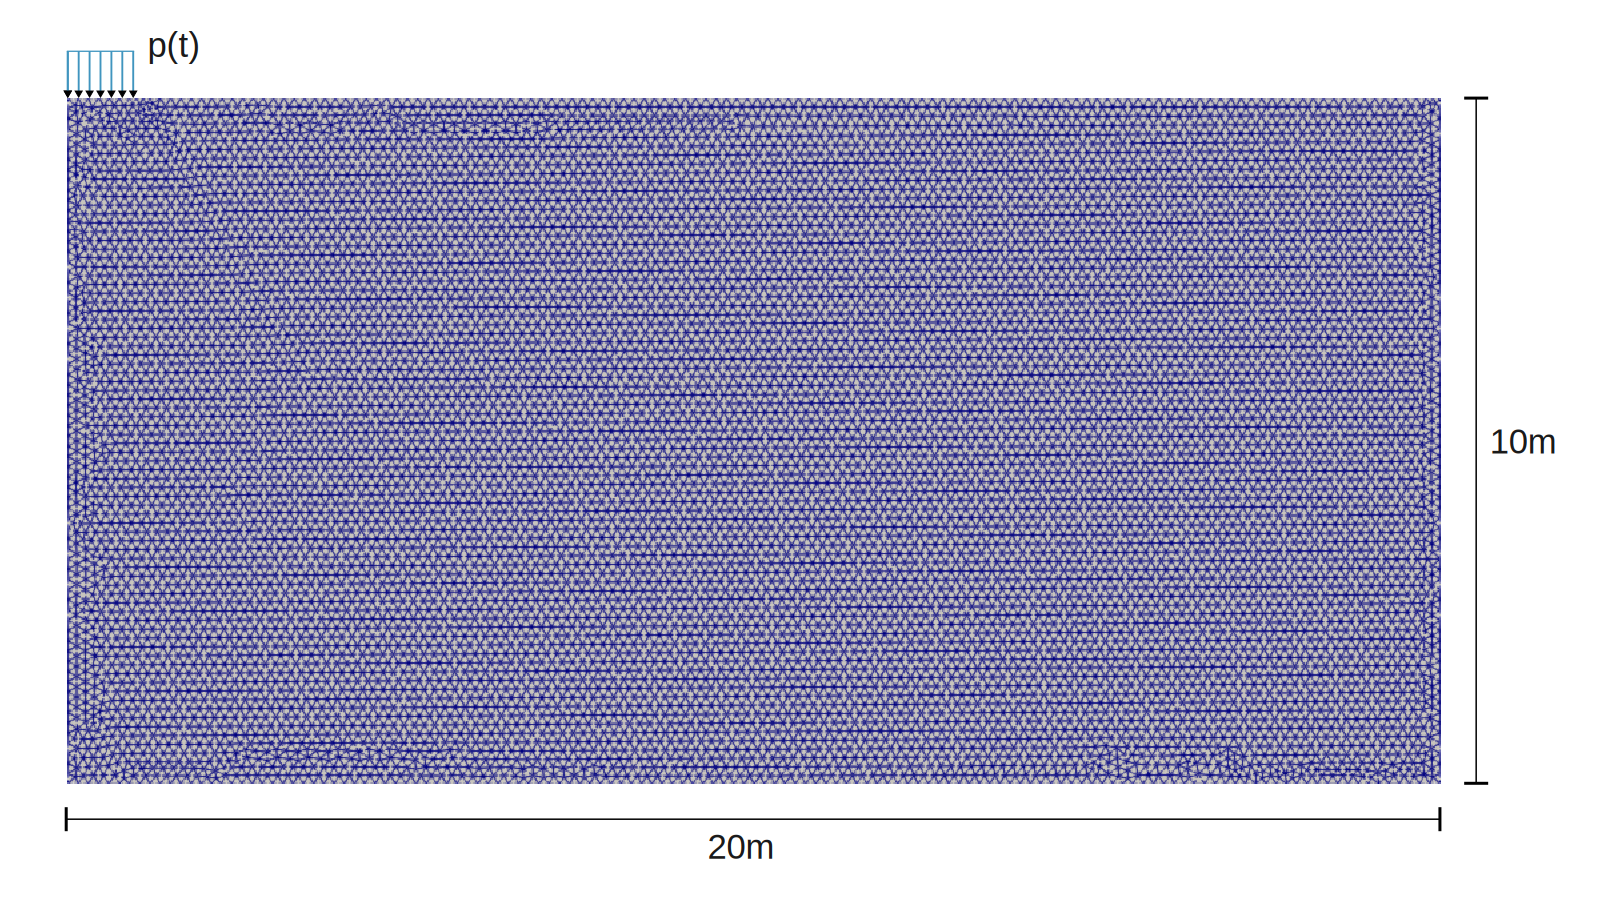
\includegraphics[width=\textwidth]{strip_load/mesh_2D.pdf}
    \caption{}
    \label{fig:strip_mesh_a}
    \end{subfigure}
    \begin{subfigure}[t]{0.49\textwidth}
        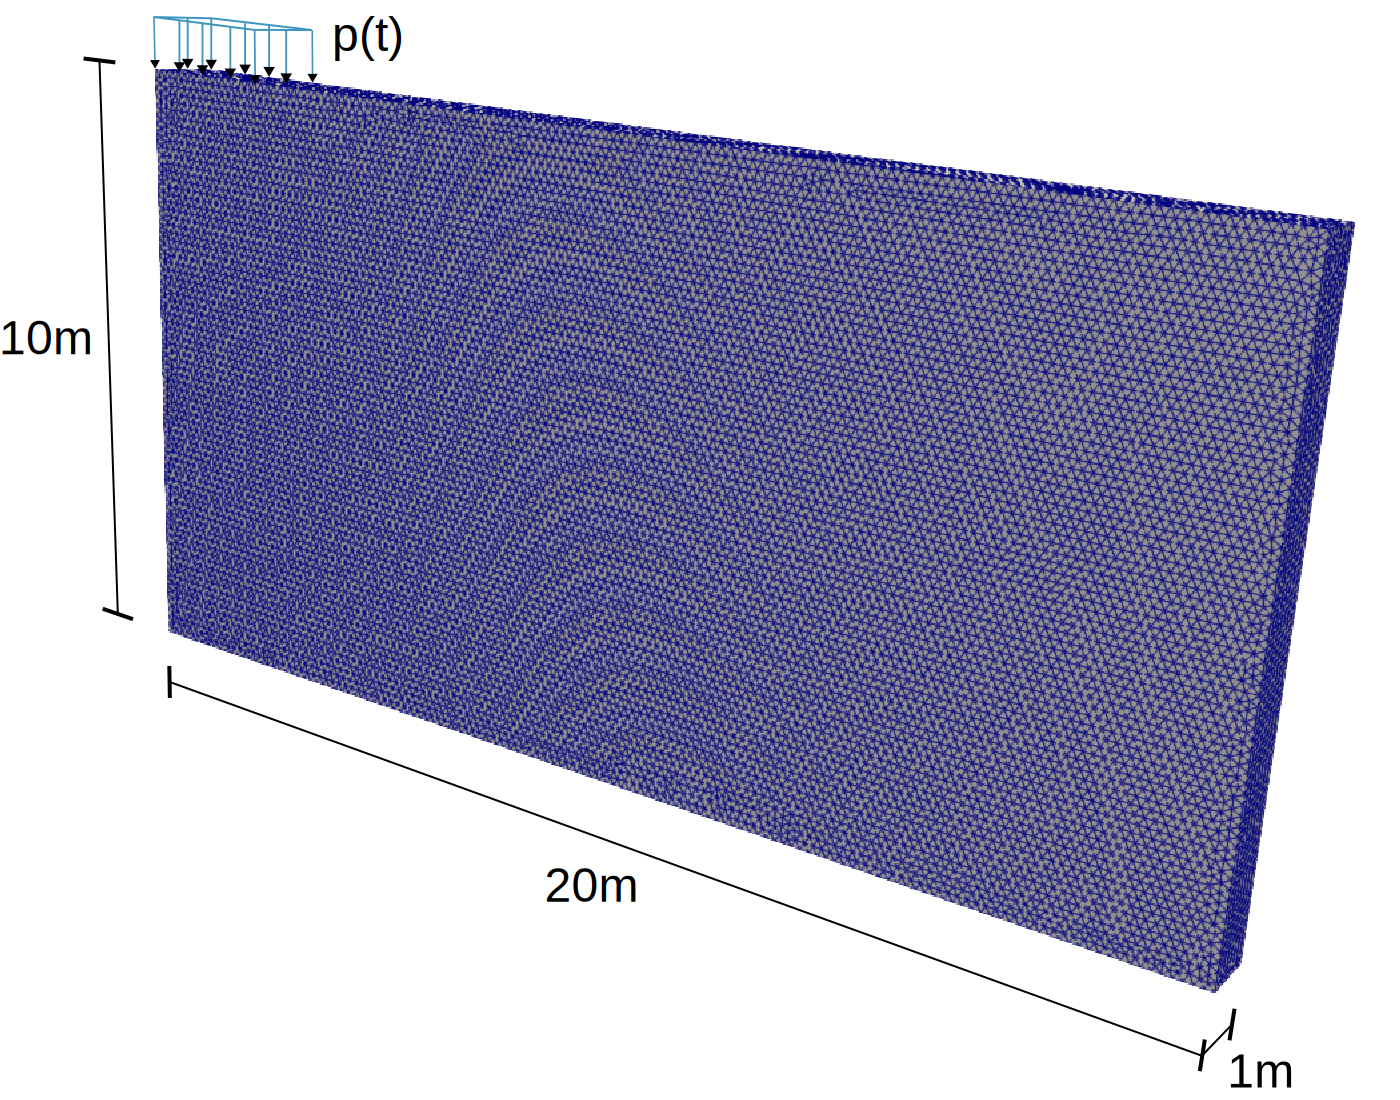
\includegraphics[width=0.8\textwidth]{strip_load/mesh_3D.pdf}
    \caption{}
    \label{fig:strip_mesh_b}
    \end{subfigure}
    \caption{Geometry and mesh for the dynamic strip load problem in: (a) two-dimensional
     and (b) three-dimensional.}
    \label{fig:strip_mesh}
\end{figure}

% ..............................................................................................
\subsection{Materials and numerical parameters}
% ..............................................................................................
The soil is modelled as a one-phase continuum with a linear elastic constitutive law, with the
following parameters:

\begin{itemize}[noitemsep,topsep=0pt,parsep=0pt,partopsep=0pt]
    \item Young's modulus: \qty{30}{\mega\pascal},
    \item Poisson ratio: 0.2,
    \item Density: \qty{2000}{\kilogram\per\meter\cubed}.
\end{itemize}

Material damping is included via Rayleigh damping, with parameters that provide a damping ratio of
\qty{2}{\percent} at \qty{1}{\hertz} and \qty{80}{\hertz}.

The dynamic analysis is performed over a \qty{0.20}{\second} time window, with a time step of \qty{0.001}{\second}.
The system of equations is solved using the Newmark time integration~\cite{Newmark_1959} scheme with
parameters $\beta = 0.25$ and $\gamma = 0.5$.

% ----------------------------------------------------------------------------------------------
\section{Results}
% ----------------------------------------------------------------------------------------------
Figure~\ref{fig:strip_results} presents the vertical stress at a depth of {\qty{1}{\meter}} below the surface,
at three moments in time: \qty{0.05}{\second}, \qty{0.075}{\second} and \qty{0.10}{\second}.
The figure compares the STEM results against the analytical solution.
If follows that there is an agreement between both solutions, demonstrating the accuracy of the STEM
for this type of dynamic loading condition.


\begin{figure}[h]
    \centering
    \includegraphics[width=0.8\textwidth]{strip_load/time_history.pdf}
    \caption{Vertical stress at a depth of {\qty{1}{\meter}} below the surface at three moments in time:
    (a) \qty{0.05}{\second}, (b) \qty{0.075}{\second} and (c) \qty{0.10}{\second}.}
    \label{fig:strip_results}
\end{figure}
